\documentclass{article}
\usepackage{graphicx}
\begin{document}

Lorem ipsum dolor sit amet, consectetuer adipiscing elit. 
Nulla nonummy sem ac nulla. Donec egestas, dolor ac laoreet volutpat, 
urna mi commodo turpis, sit amet pharetra turpis nisi sit amet elit. 
Pellentesque habitant morbi tristique senectus et netus et malesuada 
fames ac turpis egestas. Cras imperdiet, mauris et adipiscing sagittis, 
mauris turpis eleifend mauris, vel auctor lorem nulla quis lorem. 
Duis ac purus eu turpis tincidunt feugiat. Etiam eros. Vestibulum quam. 
Duis porta, odio non congue euismod, elit lacus condimentum ligula, 
vitae suscipit mi quam ut lectus. Fusce at nibh et elit pellentesque ornare. 
Nulla risus libero, sodales vel, tincidunt vel, placerat ac, massa. 
Maecenas ultricies. Vivamus id felis ac metus elementum ultricies. 
Quisque lacinia libero vel justo. Praesent iaculis massa ac arcu.

\begin{figure}
\begin{center}
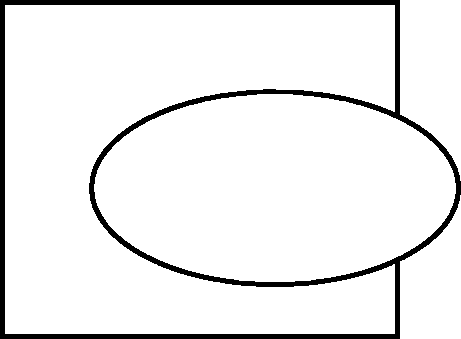
\includegraphics{fig_oval.png}
\caption{Figure size test no options.} 
\end{center}
\end{figure}

Lorem ipsum dolor sit amet, consectetuer adipiscing elit. 
Nulla nonummy sem ac nulla. Donec egestas, dolor ac laoreet volutpat, 
urna mi commodo turpis, sit amet pharetra turpis nisi sit amet elit. 
Pellentesque habitant morbi tristique senectus et netus et malesuada 
fames ac turpis egestas. Cras imperdiet, mauris et adipiscing sagittis, 
mauris turpis eleifend mauris, vel auctor lorem nulla quis lorem. 
Duis ac purus eu turpis tincidunt feugiat. Etiam eros. Vestibulum quam. 
Duis porta, odio non congue euismod, elit lacus condimentum ligula, 
vitae suscipit mi quam ut lectus. Fusce at nibh et elit pellentesque ornare. 
Nulla risus libero, sodales vel, tincidunt vel, placerat ac, massa. 
Maecenas ultricies. Vivamus id felis ac metus elementum ultricies. Q
uisque lacinia libero vel justo. Praesent iaculis massa ac arcu.

\begin{figure}
\begin{center}
\includegraphics[0,0][72,72]{fig_oval.png}
\caption{Figure size test with two options \texttt{[0,0][72,72]}.} 
\end{center}
\end{figure}

Lorem ipsum dolor sit amet, consectetuer adipiscing elit. 
Nulla nonummy sem ac nulla. Donec egestas, dolor ac laoreet volutpat, 
urna mi commodo turpis, sit amet pharetra turpis nisi sit amet elit. 
Pellentesque habitant morbi tristique senectus et netus et malesuada 
fames ac turpis egestas. Cras imperdiet, mauris et adipiscing sagittis, 
mauris turpis eleifend mauris, vel auctor lorem nulla quis lorem. 
Duis ac purus eu turpis tincidunt feugiat. Etiam eros. Vestibulum quam. 
Duis porta, odio non congue euismod, elit lacus condimentum ligula, 
vitae suscipit mi quam ut lectus. Fusce at nibh et elit pellentesque ornare. 
Nulla risus libero, sodales vel, tincidunt vel, placerat ac, massa. 
Maecenas ultricies. Vivamus id felis ac metus elementum ultricies. 
Quisque lacinia libero vel justo. Praesent iaculis massa ac arcu.

\begin{figure}
\begin{center}
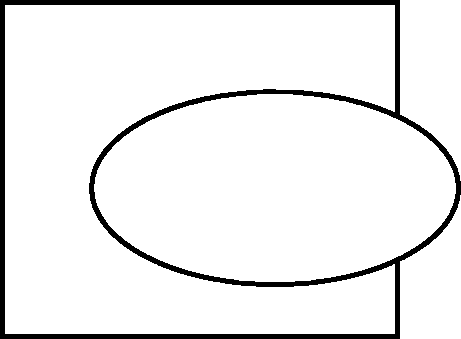
\includegraphics[scale=0.3]{fig_oval.png}
\end{center}
\caption{Figure size test with 30\% scaling.} 
\end{figure}

Lorem ipsum dolor sit amet, consectetuer adipiscing elit. 
Nulla nonummy sem ac nulla. Donec egestas, dolor ac laoreet volutpat, 
urna mi commodo turpis, sit amet pharetra turpis nisi sit amet elit. 
Pellentesque habitant morbi tristique senectus et netus et malesuada 
fames ac turpis egestas. Cras imperdiet, mauris et adipiscing sagittis, 
mauris turpis eleifend mauris, vel auctor lorem nulla quis lorem. 
Duis ac purus eu turpis tincidunt feugiat. Etiam eros. Vestibulum quam. 
Duis porta, odio non congue euismod, elit lacus condimentum ligula, 
vitae suscipit mi quam ut lectus. Fusce at nibh et elit pellentesque ornare. 
Nulla risus libero, sodales vel, tincidunt vel, placerat ac, massa. 
Maecenas ultricies. Vivamus id felis ac metus elementum ultricies. 
Quisque lacinia libero vel justo. Praesent iaculis massa ac arcu.

\begin{figure}
\begin{center}
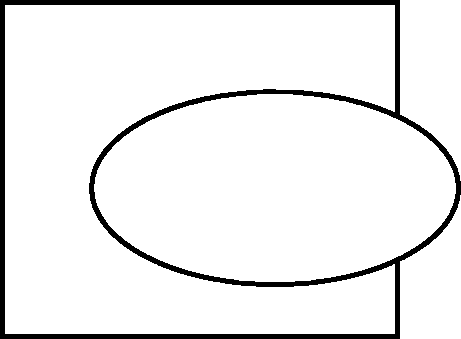
\includegraphics[scale=0.2]{fig_oval.png}
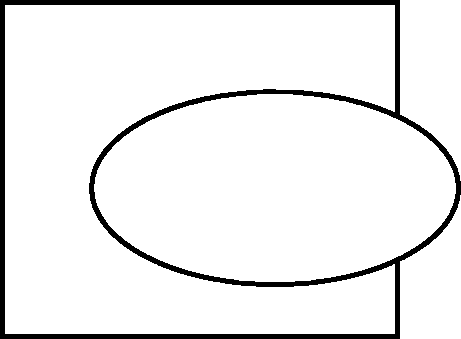
\includegraphics[scale=0.2]{fig_oval.png}
\end{center}
\caption{Two figures with 20\% scaling each.} 
\end{figure}

Lorem ipsum dolor sit amet, consectetuer adipiscing elit. 
Nulla nonummy sem ac nulla. Donec egestas, dolor ac laoreet volutpat, 
urna mi commodo turpis, sit amet pharetra turpis nisi sit amet elit. 
Pellentesque habitant morbi tristique senectus et netus et malesuada 
fames ac turpis egestas. Cras imperdiet, mauris et adipiscing sagittis, 
mauris turpis eleifend mauris, vel auctor lorem nulla quis lorem. 
Duis ac purus eu turpis tincidunt feugiat. Etiam eros. Vestibulum quam. 
Duis porta, odio non congue euismod, elit lacus condimentum ligula, 
vitae suscipit mi quam ut lectus. Fusce at nibh et elit pellentesque ornare. 
Nulla risus libero, sodales vel, tincidunt vel, placerat ac, massa. 
Maecenas ultricies. Vivamus id felis ac metus elementum ultricies. 
Quisque lacinia libero vel justo. Praesent iaculis massa ac arcu.

\begin{figure}
\begin{center}
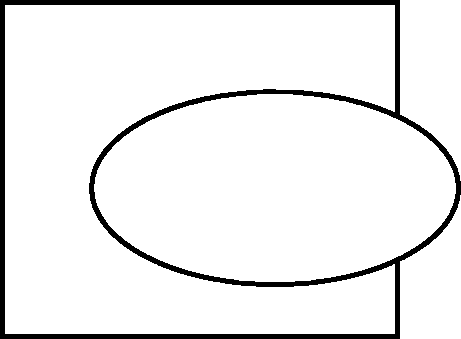
\includegraphics[width=1in,height=3cm]{fig_oval.png}
\caption{Figure size test with width of one inch and height of 3\,cm.} 
\end{center}
\end{figure}

Some poking around reveals that \verb#width=0.25\textwidth# is supported 
in \verb#getDimension()#, and appears to work correctly.  
The gotcha is that you have to explicitly specify $x$ and $y$ scaling 
in \verb#\includegraphics#; if only $x$ is specified, which is my usual 
procedure, the aspect ratio is wrong. So this works:

\begin{figure}
\begin{center}
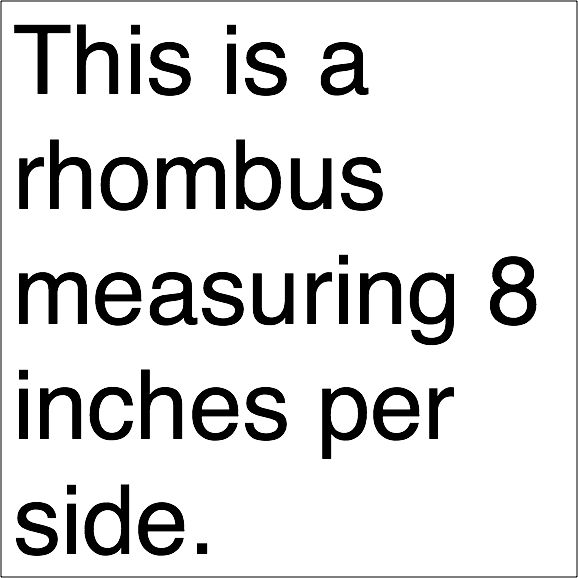
\includegraphics[width=0.25\textwidth,height=0.25\textwidth]{fig_testf.png}
\end{center}
\caption{Figure size test with width and height equal to one quarter of text width.} 
\end{figure}

The following used to fail.

\begin{figure}
\begin{center}
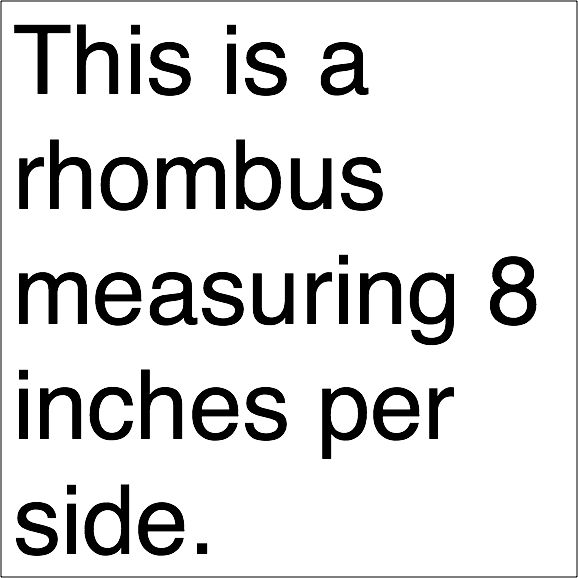
\includegraphics[width=0.25\textwidth]{fig_testf.png}
\caption{Figure size test with width set to one quarter of text width.} 
\end{center}
\end{figure}

Test that height also works properly
\begin{figure}
\begin{center}
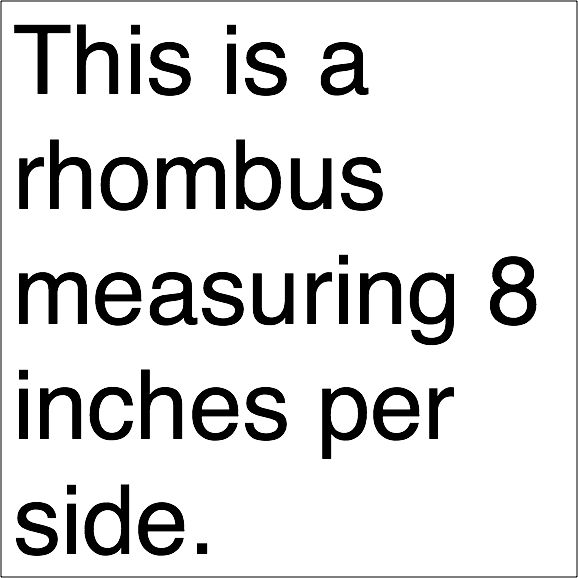
\includegraphics[height=0.25\textwidth]{fig_testf.png}
\caption{Figure size test with height set to one quarter of text width.} 
\end{center}
\end{figure}

\end{document}
